\section{Languages that are and are not Regular}

The regular languages are closed under a variety of operations and that regular languages may be specified either by regular expressions or by deterministic or nondeterministic finite automata. These facts, used singly or in combinations, provide a variety of techniques for showing languages to be regular.

\begin{example}{}
  Let $\Sigma = \{0, 1, ..., 9\}$ and let $L \subseteq \Sigma^*$ be the set of decimal representations for nonnegative integers (without redundant leading O's) divisible by 2 or 3. For example, $0, 3, 6, 244 \in L$, but $1, 03, 00 \notin L$. Then $L$ is regular. We break the proof into four parts.

  \quad Let $L_1$ be the set of decimal representations of nonnegative integers. Then it is easy to see that
  \begin{equation*}
    L_1 = 0 \cup \left\{ 1, 2, ..., 9 \right\} \Sigma^*
  \end{equation*}
  which is regular since it is denoted by a regular expression.

  \quad Let $L_2$ be the set of decimal representations of nonnegative integers divisible by 2. Then $L_2$ is just the set of members of $L$, ending in 0, 2, 4, 6, or 8; that is,
  \begin{equation*}
    L_2 = L_1 \cap \Sigma^* \left\{ 0, 2, 4, 6, 8 \right\}
  \end{equation*}
  which is regular by Theorem 2(e).

  \quad Let $L_3$ be the set of decimal representations of nonnegative integers divisible by 3. Recall that a number is divisible by 3 if and only if the sum of its digits is divisible by 3. We construct a finite automaton that keeps track in its finite control of the sum modulo 3 of a string of digits. $L_3$ will then be the intersection with $L_1$ of the language accepted by this finite automaton. The automaton is pictured in Figure 15.

  \quad Finally, $L = L_2 \cup L_3$ , surely a regular language.
\end{example}

\begin{figure}[h!]
  \centering
  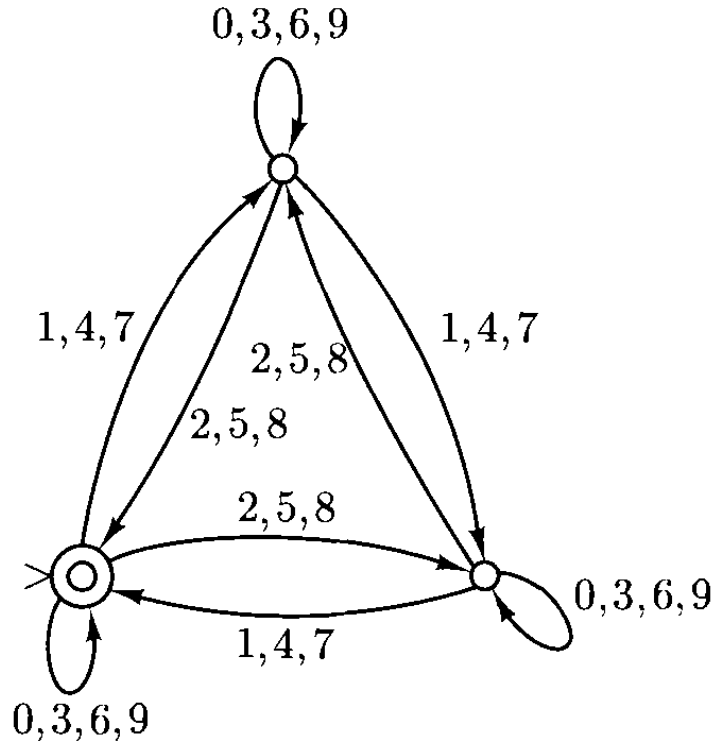
\includegraphics[width=.3\textwidth]{img/Fig2.18.png}
  \caption{}
\end{figure}

\begin{formula}{From Ebru Hoca's Notes}
  To show that a language $L$ is regular, one of the following methods can be used:
  \begin{itemize}
    \item write a regular expression $\alpha$ such that $L = L(\alpha)$
    \item construct an NFA $M$ such that $L = L(M)$
    \item use closure properties, e.g., for regular languages $L_1$ and $L_2$, show $L = L_1 \cap L_2$, $L = L_1 \cup L_2$, $L = L_1 L_2$,
    or $L = \Sigma^* \setminus L_1$ (more examples can be added)
  \end{itemize}
\end{formula}

Although we now have a variety of powerful techniques for showing that languages are regular, as yet we have none for showing that languages are not regular. Two properties shared by all regular languages, but not by certain nonregular languages, may be phrased intuitively as follows: 
\begin{enumerate}
  \item As a string is scanned left to right, the amount of memory that is required in order to determine at the end whether or not the \textit{string is in the language must be bounded}, fixed in advance and dependent on the language, not the particular input string. For example, we would expect that $\{a^n b^n\ |\ n \geq 0\}$ is not regular, since it is difficult to imagine how a finite-state device could be constructed that would correctly remember, upon reaching the border between the $a$'s and the $b$'s, how many $a$'s it had seen, so that the number could be compared against the number of $b$'s.
  \item Regular languages with an infinite number of strings are represented by automata with cycles and regular expressions involving the Kleene star. Such languages must have infinite subsets with a certain simple repetitive structure that arises from the Kleene star in a corresponding regular expression or a cycle in the state diagram of a finite automaton. This would lead us to expect, for example, that $\{a^n\ |\ n \geq 1 \textnormal{ is a prime}\}$ is not regular, since there is no simple periodicity in the set of prime numbers.
\end{enumerate}

In brief,
\begin{formula}{From Ebru Hoca's Notes}
  To show that a language $L$ is not regular, we use the following property of regular languages: 
  \begin{itemize}
    \item as a string is scanned from left to right, the amount of memory required to determine if $w \in L$ or $w \notin L$ must be bounded.
    \item In RL, infinite languages can be represented with Kleene star (cycle in automata), which induce a periodicity/pattern.
  \end{itemize}
\end{formula}

These intuitive ideas are formalized in the following theorem known as \textit{Pumping Lemma}.

\begin{theorem}{: Pumping Lemma}
  \textit{Let $L$ be a regular language. There is an integer $n \geq 1$ such that any string $w \in L$ with $|w| \geq n$ can be rewritten as $w = xyz$ such that $y \neq e$, $|xy| \leq n$ and $xy^iz \in L$ for each $i \geq 0$.}  
\end{theorem}

\begin{proof}
  Since $L$ is regular, $L$ is accepted by a deterministic finite automaton $M$. Suppose that $n$ is the number of states of $M$, and let $w$ be a string of length $n$ or greater. Consider now the first $n$ steps of the computation of $M$ on $w$:
  \begin{equation*}
    \left( q_0, w_1w_2...w_n \right) \vdash_M \left( q_1, w_2...w_n \right) \vdash_M ... \vdash_M (q_n, e)
  \end{equation*}
  where $q_0$ is the initial state of $M$, and $w_1...w_n$ are the $n$ first symbols of $w$. Since $M$ has only $n$ states, and there are $n + 1$ configurations $(q_i, w_{i+1}..., w_n)$ appearing in the computation above, by the \textit{pigeonhole principle} there exist $i$ and $j$, $0 \leq i < j \leq n$, such that $q_i = q_j$. That is, the string $y = w_iw_{i+1}...w_j$ drives $M$ from state $q_i$ back to state $q_i$, and this string is nonempty since $i < j$. But then this string could be removed from $w$, or repeated any number of times in $w$ just after the $j$th symbol of $w$, and $M$ would still accept this string. That is, $M$ accepts $xy^iz \in L$ for each $i \geq 0$, where $x = w_1...w_i$, and $z = w_{j+1}...w_m$. Notice finally that the length of $xy$, the number we called $j$ above, is by definition at most $n$, as required.

  Also, watch the following video: \href{https://youtu.be/qtnNyUlO6vU}{What is the Pumping Lemma}

  \begin{formula}{}
    \quad Assume $L$ is a regular language and there is a string $w \in L$. Now, imagine, not find or determine, that there is a integer $n$ that is $n \geq 1$, $n > 0$. Also, this integer is smaller than the length of the string $w$, $n \leq |w|$. So,
  \begin{align*}
    |w| \geq n \geq 1 && \textnormal{or} && |w| \geq n > 0
  \end{align*}
  Also, notice that the string can be written as three parts: $w = xyz$.

  If the followings are satisfied, it shows that $w \in L$ and $L$ is regular:
  \begin{itemize}
    \item $|y| > 0$: $y$ is not empty string
    \item $|xy| \leq n$: the length of the part of the string $xy$ is less than $n$
    \item $xy^iz \in L,\textnormal{ for each } i \geq 0$: When part $y$ is repeated, or pumped, as many times we want, the expression is still in language
  \end{itemize}
  In here, $x$ or $z$ can be empty string, $e$, but $y$ cannot be the empty string, $e$. Notice that the chosen part of string that will be compared with $n$ should be located in first $n$.
  \end{formula}
\end{proof}

Pumping lemma is also used to show that a language is not regular: start applying the pumping lemma, then find a contradiction.
\begin{formula}{}
\noindent For each regular language $L$,

\quad there exists $n \geq 1$ such that (this is a general term do not pick a number!!!)

\quad \quad for each $w \in L$ with $|w| \geq n$ (write a string with respect to $n$, that can be used to reach a contradiction)

\quad \quad \quad there exists $x, y, z$ with $w = xyz$, $y \neq e$, $|xy| \leq n$ (consider each possible split satisfying these constraints)

\quad \quad \quad \quad for each $i \geq 0$, $xy^iz \in L$ (show that there exists an $i$ such that $xy^iz \neq L$, contradiction)
\end{formula}

Applying the theorem correctly can be subtle. It is often useful to think of the application of this result as a \textit{game} between yourself, the prover, who is striving to establish that the given language $L$ is not regular, and an adversary who is insisting that $L$ is regular. 

\begin{formula}{}
\noindent The theorem states that, once $L$ has been fixed,

\quad the adversary must start by providing a number $n$;

\quad \quad then you come up with a string $w$ in the language that is longer than $n$, $|w| \geq n$;

\quad \quad \quad the adversary must now supply an appropriate decomposition of $w$ into $xyz$;

\quad \quad \quad \quad and, finally, you triumphantly point
out $i$ for which $xy^iz$ is not in the language.
\end{formula}

If you have a strategy that always wins, no matter how brilliantly the adversary plays, then you have established that $L$ is not regular.

\begin{example}{}
  The language $L = \{a^ib^i\ |\ i \geq 0\}$ is not regular, for if it were regular, Theorem 4 would apply for some integer $n$. Consider then the string $w = a^nb^n \in L$. By the theorem, it can be rewritten as $w = xyz$ such that $|xy| \leq n$ and $y \neq e$ -that is, $y = a^i$ for some $i > 0$. But then $xz = a^{n-i}b^n \notin L$, $y^0 = e$, contradicting the theorem.
\end{example}

\begin{example}{}
  The language $L = \{a^n\ |\ n \textnormal{ is prime}\}$ is not regular. For suppose it were, and let $x$, $y$, and $z$ be as specified in Theorem 4. Then $x = a^p$ , $y = a^q$, and $z = a^r$, where $p, r \geq 0$ and $q > 0$. By the theorem, $xy^iz \in L$ for each $i \geq 0$; that is, $p + iq + r$ is prime for each $i \geq 0$. But this is impossible; for let $i = p + 2q + r + 2$; then $p + iq + r = (q + 1) \cdot (p + 2q + r)$, which is a product of two natural numbers, each greater than 1.
\end{example}

\begin{example}{}
  Sometimes it pays to use closure properties to show that a language is not regular. Take for example
  \begin{equation*}
    L = \left\{ w \in \left\{ a, b \right\}^*\ |\ w \textnormal{ has an equal number of $a$'s and $b$'s} \right\}
  \end{equation*}
  $L$ is not regular, because if $L$ were indeed regular, then so would be $L \cap a^*b^*$ -by closure under intersection. However, this latter language is precisely ${a^nb^n\ |\ n \geq 0}$, which we just showed is not regular.
\end{example}
